\documentclass[12pt,a4paper]{article}
\usepackage{hyperref}
\usepackage{graphicx}
\usepackage{epstopdf}
\usepackage[section]{placeins}

\title{Finding Optimized Machine Learning Model For Recognizing English Handwritten Digit}
\author{Nowfel Mashnoor\\Roll: 1503069\and Amir Faruk\\Roll: 1503075}

\begin{document}
\date{}
\maketitle

\begin{abstract}
This paper is about the comparison between different Machine Learning models(classifiers) trained and tested on MNIST dataset. For declaring a model as best, we only considered low error score. A standard machine learning library written in Python Programming Language is used during this research. 
\end{abstract}

\section{Introduction}

Handwritten Digit Recognition has been very successful in recent years. A lot of research and studies has been done in recent years on it like Devnagari Handwritten Character Recognition\cite{pal2009comparative}. Handwritten digit recognition technique is used in various fields like PDA, bank cheque, handwritten fields in form etc.\cite{plamondon2000online} Using machine learning technique, which which can be briefly defined as enabling computers make successful predictions using past experiences, \cite{bacstanlar2014introduction} handwritten digit recognition system is greatly improved. Handwritten Digit recognition is a supervised learning algorithm problem. There are many classifier in supervised learning like Neural Network, Decision Tree,  Bayesian Network, Support Vector Machine(SVM), Random Forest etc\cite{kotsiantis2007supervised}. A comparison study has been already done where \textit{Base Linear Classifier, Baseline Nearest Neighbor Classifier, Large Fully Connected Multi-Layer Neural Network, Tangent Distance Clasifier(TDC), LeNet 4 With KNN, Optimal Margin Classifier} are compared among.\cite{lecun1995learning} In our research we are going to compare among algo1, algo2, algo3. We will chose the best classifier among them based on their accuracy on testing set. 

\section{MNIST Dataset}

For training and testing our classifiers, we used MNIST (Modified National Institute of Standards and Technology) Dataset. This dataset contains \textit{70000} images. Among 70000 images, 60000 images are for training and 10000 images are for testing\cite{kussul2004improved}.  It is basically a subset of NIST dataset. the black and white images from NIST were normalized to fit into a 28x28 pixel and converter to grayscale levels.\cite{lecuncourant}

\begin{figure}[!htb]
  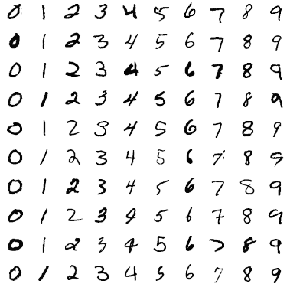
\includegraphics[width=5cm,height=5cm,keepaspectratio]{mnist_example.png}
  \centering
  \caption{MNIST Dataset Sample Images}
  \label{fig:mnist_sample}
\end{figure}
For each and every classifier we are using in our study, we will use use all the 60000 images for training and the rest 10000 images for evaluating our models. 

\section{Scikit Learn Machine Learning Library}
Scikit-learn is a Python module integrating a wide range of state-of-the-art machine learning algorithms for medium-scale supervised and unsupervised problems\cite{pedregosa2011scikit}. Most of the algorithms are written in Python programming language where some of the algorithms are written in Cython for achieving optimal performance. Also for efficient operation on large arrays and multidimensional matrices, we used NumPy library.\cite{walt2011numpy} For graphing and other visualization purpose, we used Matplotlib, which is other Python Library. \cite{hackeling2014mastering} For training and testing our classifiers, we will use the Scikit Learn Library. This library also provides tools for model evaluation. 


\section{The Classifiers}
We have trained and tested three classifiers on MNIST Dataset. We are going to give a quick and brief description of all of them. 
\subsection{Random Forest}
Random Forest is a powerful Machine Learning model. It can do both regression and classification.\cite{liaw2002classification} It is basically a collection of random decision trees. Each decision tree predict a class and after all the prediction, random forest outputs that class which got the most vote. The main benefit of Random Forest over decision tree is that it removes the problem of over fitting of decision tree.\cite{friedman2001elements} 
\begin{figure}[!htb]
  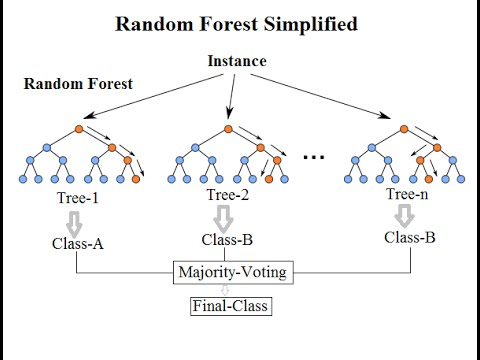
\includegraphics[width=10cm,height=10cm,keepaspectratio]{random_forest.jpg}
  \centering
  \caption{Random Forest}
  \label{fig:random_forest}
\end{figure}
Random forest uses Bootstrap aggregating or Tree Bagging algorithm. It reduces variance and helps to prevent over fitting. In decision tree learning, for splitting the variable at each step, different metrics can be used like Gini Impurity, Information Gain. We used Gini Index or Gini Impurity in our work. For calculating Gini Index, we have to use the following formula: \\
\centerline{$I_{G}(P)$ = $\sum_{i=1}^{J}p_{i}\sum_{k\neq{i}}p_{k}$}
Where,\\
J = No. of Classes\\
i $\epsilon$ {1, 2, 3, ..., J}\\
$p_{i}$ = Probability of an item with label \textit{i} being chose\\
$p_{k}$ = Probability of a mistake categorizing that item \cite{wiki:decisiontreelearning}
 
\bibliography{ref} 
\bibliographystyle{ieeetr}

\end{document} 